\documentclass[letterpaper, 6 pt, journal, twoside]{IEEEtran}
\usepackage[utf8]{inputenc}
\usepackage{amsmath}
\usepackage{graphicx}
\usepackage[colorlinks=true, allcolors=blue]{hyperref}
\usepackage[capitalize]{cleveref}

\begin{document}

\begin{figure}
    \centering
    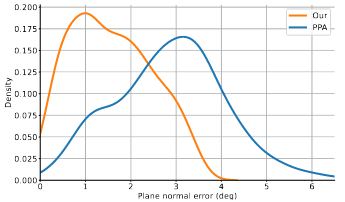
\includegraphics{images/Figure_3.png} 
    \caption{Plane normal error distributions for our method and PPA.}
    \label{fig:Fig3}
\end{figure}

effect is strongly attenuated, showing evidence that the per-
spective distortion have been effectively compensated. PPA
performs better than Ortho, but the radial pattern is still par-
tially visible.

\subsection{Plane orientation estimation}

    Since in the Orthographic model $\phi$ is the azimuth angle of $\Vec{n}$, the linear constraint 
\begin{equation}
        (\begin{array}{ccc} \sin{\phi} & \cos{\phi} & 0 \end{array}) . \Vec{n} = 0
\end{equation}

is usually considered in photo-polarimetric stereo ap-
proaches or iso-depth contour tracing. If we know that at
least K $>$ 3 pixels observe the same plane, we can use such
constraint to recover the plane normal $\Vec{n}$ (in camera refer-
ence frame) from the (corrected) $\phi_j$ observed at each pixel
by solving:

\begin{equation}
        (\begin{array}{cccc} 
        (\sin{\phi_1} & \cos{\phi_1} & 0 ) & R_1^T \\
        (\sin{\phi_2} & \cos{\phi_2} & 0 ) & R_2^T \\
        & . \\
        & . \\
        & . \\
        (\sin{\phi_K} & \cos{\phi_K} & 0 ) & R_K^T \\
        \end{array})  
        \Vec{n} = \Vec{0}
\end{equation}

as a Linear Least-Squares problem. Note that the system is
under-determined in the Orthographic model because all the
rays are parallel ($R_1 , . . . R_k$ are identities) and all the pixels
would observe the same $\phi$. In the PPA model, instead, a
similar costraint is provided (See Eq. 7 in \cite{chen2022perspective}).
In \cref{fig:Fig3} we plotted the the estimated plane normal er-
ror distribution against the Ground Truth data in the PPA
dataset. The Ortho model is not present in the plot for the
reasons discussed before. Also in this case, our mean abso-
lute error is lower (1.57\textdegree vs. 2.89\textdegree) and with less variabil-
ity. This reflects a better estimation of the AoLP due to the
correction applied by the tilted polarizer model.

{\small
\bibliographystyle{IEEEtran}
\bibliography{Ref}
}

\end{document}
